% l4h user manual.  Build with `make -C docs/manual` (needs TeX Live and
% latexmk); the PDF is a build product and is not committed.
\documentclass[11pt,a4paper]{report}

\usepackage[T1]{fontenc}
\usepackage{lmodern}
\usepackage{microtype}
\usepackage[margin=2.6cm]{geometry}
\usepackage{xcolor}
\usepackage{listings}
\usepackage{booktabs}
\usepackage{tabularx}
\usepackage{longtable}
\usepackage{enumitem}
\usepackage{tikz}
\usetikzlibrary{positioning,fit,arrows.meta}
\usepackage[hidelinks]{hyperref}

\definecolor{codebg}{gray}{0.95}
\definecolor{note}{RGB}{0,70,140}
\lstset{
  basicstyle=\ttfamily\small,
  backgroundcolor=\color{codebg},
  frame=none,
  columns=fullflexible,
  keepspaces=true,
  showstringspaces=false,
  breaklines=true,
  aboveskip=0.8em,
  belowskip=0.8em,
  xleftmargin=0.5em,
  xrightmargin=0.5em,
  upquote=true,
}
\newcommand{\cmd}[1]{\texttt{#1}}
\newcommand{\file}[1]{\texttt{#1}}
\newenvironment{caveat}{\par\medskip\noindent\color{note}\textbf{Note.}\ }{\par\medskip}
\setlist{itemsep=0.2em}
\setlength{\emergencystretch}{3em}

\title{\Huge l4h User Manual\\[0.5em]\Large A paravirtual hypervisor for Linux on seL4}
\author{The l4h project}
\date{Version 0.1 (\today)}

\begin{document}
\maketitle
\tableofcontents

%======================================================================
\chapter{Introduction}

l4h runs Linux virtual machines on the seL4 microkernel. It uses
\emph{no hardware virtualization} (no VT-x, no EL2) and emulates no
instructions. Instead, each guest runs a paravirtualized Linux kernel,
\texttt{ARCH=l4h}, derived from user-mode Linux. A guest's processes are
ordinary seL4 threads and address spaces, and its devices are virtio devices
served by host components. Because nothing depends on virtualization
extensions, l4h runs anywhere seL4 runs, including cloud VMs that do not
offer nested virtualization.

This manual is for people who build, deploy and operate an l4h host. It
covers:
\begin{itemize}
  \item building the hypervisor, the guest kernel and the tools
        (Chapter~\ref{ch:build});
  \item configuring and booting a host, on QEMU or from a UEFI disk image
        for Google Compute Engine (Chapters~\ref{ch:dom0} and~\ref{ch:boot});
  \item managing VMs, disks, switches and CPU from dom0 with \cmd{l4hctl}
        (Chapters~\ref{ch:l4hctl}--\ref{ch:cpu});
  \item recovery, troubleshooting and the test suite
        (Chapters~\ref{ch:recovery}--\ref{ch:tests}).
\end{itemize}
The design and the reasons behind it are in \file{DESIGN.md} in the source
tree, which also records the status of every part.

\section{Concepts}

\begin{description}
  \item[Host.] The machine l4h runs on: a physical machine, a QEMU VM or a
    cloud VM. It provides CPU cores, memory, PCI disks (virtio-blk, virtio-scsi or NVMe)
    and PCI NICs (virtio-net).
  \item[Guest, or VM.] A Linux system running on l4h. Every guest has a
    name, a numeric id, a number of vCPUs, a fixed amount of RAM, and up to
    16 devices: a console, disks and network interfaces.
  \item[dom0.] The first guest, id 0. It is an ordinary guest with one
    extra device, \file{/dev/l4hctl}, through which it controls the host. Its
    kernel, initramfs and settings sit next to the host image, on its EFI
    system partition (or, under QEMU, are appended to it). dom0 decides
    what runs, but it cannot read other guests' memory, and it runs no device
    drivers for host hardware.
  \item[Disk.] A host block device, numbered from 0 in PCI order. A disk is
    \emph{passed through} to exactly one guest, either whole or as a window
    of sectors, optionally read-only. There are no image files and no host
    filesystem.
  \item[Switch.] An L2 Ethernet switch, numbered from 0. Switches learn MAC
    addresses and flood unknown traffic. Each switch is its own broadcast
    domain.
  \item[NIC.] A host network card, numbered from 0. A NIC can be the
    \emph{uplink} of one switch: it becomes a port of that switch, and frames
    are switched to and from it like any other port.
  \item[vNIC.] A guest network interface. Each vNIC is a port on exactly one
    switch and appears in the guest as \texttt{eth}$N$.
  \item[Router VM.] l4h itself only switches Ethernet frames. Routing, NAT,
    DHCP and firewalls run in a guest of your choice, with standard Linux
    tools.
\end{description}

\section{Architecture}

Figure~\ref{fig:arch} shows the components of a running host. All of them
are seL4 user-level programs; only the seL4 kernel runs privileged.

\begin{figure}[ht]
\centering
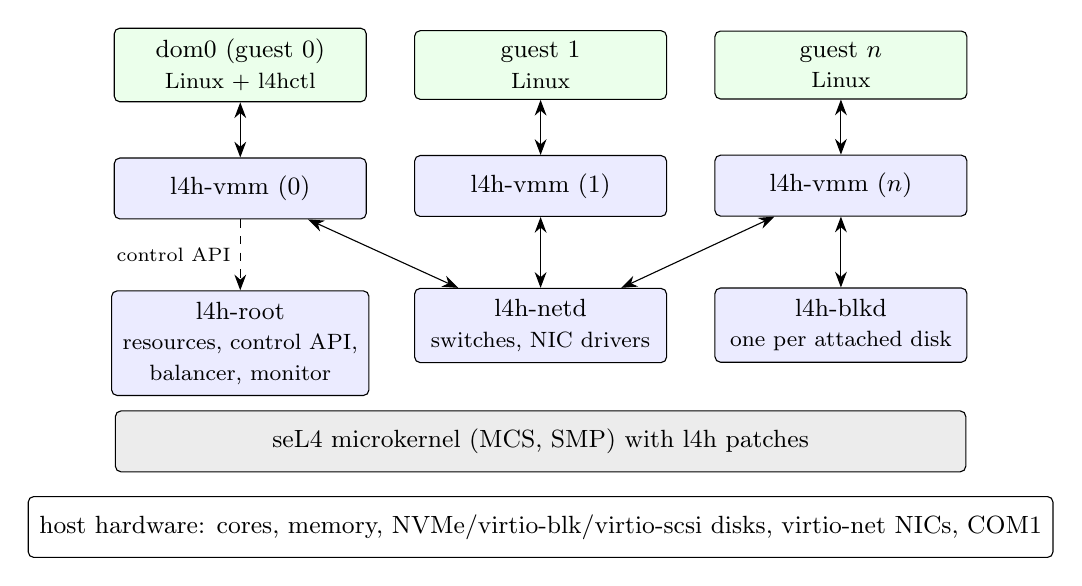
\begin{tikzpicture}[
  box/.style={draw, rounded corners=2pt, align=center, minimum height=2.2em, inner sep=4pt, font=\small},
  host/.style={box, fill=blue!8},
  guest/.style={box, fill=green!8},
  >={Stealth[length=2mm]}]
  \node[guest, minimum width=3.2cm] (dom0) {dom0 (guest 0)\\\footnotesize Linux + l4hctl};
  \node[guest, minimum width=3.2cm, right=0.6cm of dom0] (ga) {guest 1\\\footnotesize Linux};
  \node[guest, minimum width=3.2cm, right=0.6cm of ga] (gb) {guest $n$\\\footnotesize Linux};
  \node[host, below=0.7cm of dom0, minimum width=3.2cm] (v0) {l4h-vmm (0)};
  \node[host, below=0.7cm of ga, minimum width=3.2cm] (va) {l4h-vmm (1)};
  \node[host, below=0.7cm of gb, minimum width=3.2cm] (vb) {l4h-vmm ($n$)};
  \node[host, below=0.9cm of v0, minimum width=3.2cm] (root) {l4h-root\\\footnotesize resources, control API,\\\footnotesize balancer, monitor};
  \node[host, below=0.9cm of va, minimum width=3.2cm] (netd) {l4h-netd\\\footnotesize switches, NIC drivers};
  \node[host, below=0.9cm of vb, minimum width=3.2cm] (blkd) {l4h-blkd\\\footnotesize one per attached disk};
  \node[box, below=0.6cm of netd, minimum width=10.8cm, fill=gray!15] (k) {seL4 microkernel (MCS, SMP) with l4h patches};
  \node[box, below=0.3cm of k, minimum width=10.8cm] (hw) {host hardware: cores, memory, NVMe/virtio-blk/virtio-scsi disks, virtio-net NICs, COM1};
  \foreach \g/\v in {dom0/v0, ga/va, gb/vb} \draw[<->] (\g) -- (\v);
  \draw[->, dashed] (v0) -- node[left, font=\scriptsize] {control API} (root);
  \draw[<->] (v0) -- (netd); \draw[<->] (va) -- (netd); \draw[<->] (vb) -- (netd);
  \draw[<->] (vb) -- (blkd);
\end{tikzpicture}
\caption{Components of an l4h host.}
\label{fig:arch}
\end{figure}

\begin{description}
  \item[seL4] with fourteen l4h patches (\file{kernel/patches}): trapping guest
    system calls, FPU state access, per-thread deadline timers and a few
    fixes.
  \item[l4h-root] is the root task. It owns the devices, creates and
    destroys guests, executes control-API requests, balances vCPUs across
    cores, and runs the serial monitor.
  \item[l4h-memd] owns the free memory and every guest's RAM. The root task
    gets the memory for its own objects from it, and it reports free
    memory to the hypervisor when l4h runs in a VM.
  \item[l4h-vmm] runs once per guest. It serves the guest's hypercalls and
    virtio devices. It maps only its own guest's I/O pool (below), never its
    RAM, so a compromised VMM can harm only that guest.
  \item[l4h-blkd] runs once per attached disk. It drives the disk (virtio-blk,
    virtio-scsi or NVMe), checks every request against the guest's I/O pool and its
    sector window, and lets the device DMA straight into the pool.
  \item[l4h-netd] holds every switch and drives the uplink NICs.
\end{description}

\paragraph{Trust.} The seL4 kernel, \texttt{l4h-root}, \texttt{l4h-memd},
\texttt{l4h-blkd} and \texttt{l4h-netd} are trusted by everyone. dom0 is trusted to decide what
runs, and nothing more. Guest kernels are untrusted, and capabilities confine
them. The trusted drivers validate every DMA address, and guests never touch
device registers. On an AMD or Intel host with a supported IOMMU, \texttt{l4h-root} also confines every
device with the IOMMU to the memory it was given (the setting
\texttt{iommu}); elsewhere nothing confines a device.

\paragraph{The I/O pool.} Each guest has a small I/O pool, 4~MiB by
default, that belongs to the host and is mapped into the guest after its
RAM. All device I/O goes through it: the guest kernel copies data between
its own pages and the pool with Linux's standard restricted-DMA (swiotlb)
mechanism, and devices, \texttt{l4h-vmm} and the drivers access only the
pool. The VMM refuses any virtio ring, descriptor or buffer outside it,
and a guest kernel that does not accept
\texttt{VIRTIO\_F\_ACCESS\_PLATFORM} gets no devices.

\section{Status and limitations}

This is version 0.1. Before you depend on it, note the following.
\begin{itemize}
  \item Linux guests run on x86\_64 and AArch64. The AArch64 platform
        is QEMU \texttt{virt} with GICv2m, including SMP, PCI virtio disks
        and NICs, NVMe, the RTC and serial monitor. QEMU virtualization
        is disabled; the loader starts directly at EL1.
  \item The UEFI image has been tested locally under QEMU with OVMF and on
        GCE \texttt{n2-standard-4} instances with virtio-net. gVNIC,
        which C3, C4 and N4 machines require, is not supported.
  \item There is no pause or resume, live migration, memory ballooning,
        multi-queue disks, discard, I/O rate limits or VLANs.
  \item Disk and NIC configuration is fixed when a VM is created: there is
        no hotplug.
  \item Guest RAM is reserved in full when a VM is created. Memory is not
        overcommitted, although CPU is.
\end{itemize}

%======================================================================
\chapter{Building}
\label{ch:build}

\section{Requirements}

A Linux x86\_64 build machine with:
\begin{itemize}
  \item gcc, make, cmake, ninja, git, and the Python modules seL4's build
        needs, installed in a virtual environment at \file{.venv} in the
        source tree;
  \item Rust: a stable toolchain, plus the nightly toolchain pinned in
        rust-sel4's
        \file{rust-\allowbreak toolchain.toml};
  \item the usual Linux kernel build dependencies (flex, bison, bc,
        libelf, OpenSSL headers);
  \item QEMU (\texttt{qemu-system-x86\_64}) with KVM, to run hosts locally;
  \item a static busybox, cpio and e2fsprogs, for initramfs and disk images;
  \item for UEFI images: GRUB EFI (\texttt{grub-efi-amd64-bin}), mtools,
        sfdisk and OVMF;
  \item for Debian guests: debootstrap and sudo;
  \item for aarch64: \texttt{gcc-aarch64-linux-gnu}, cross libc headers,
        \texttt{qemu-system-arm} and a static AArch64 BusyBox.
        \cmd{tools/ci-setup.sh aarch64} prepares these on Debian 13.
\end{itemize}
KVM serves only as a fast CPU for QEMU. The run scripts hide VMX from the
emulated machine, so seL4 runs exactly as it would on a cloud VM without
nested virtualization.

\section{Sources}

\begin{lstlisting}[language=bash]
git clone <l4h repository> l4h && cd l4h
git submodule update --init      # seL4, rust-sel4, sDDF, kemu
python3 -m venv .venv && .venv/bin/pip install sel4-deps   # seL4's build tools
\end{lstlisting}

Linux itself is not a submodule. Extract a Linux 6.18 tree into
\file{build/linux-6.18}. The build links \file{guest/linux/arch/l4h} into it
and imports kemu's patches and source overlay before applying
\file{guest/linux/patches}. Applied patch copies and an overlay checksum
allow repeated builds and updates without extracting Linux again.
The x86\_64 guest build also needs Rust's \texttt{rust-src} component,
Clang/libclang and \texttt{bindgen-cli} 0.71.1; \cmd{tools/ci-setup.sh}
installs them.

\section{AArch64}

Build seL4 and the loader once, then set \texttt{L4H\_ARCH=aarch64}
for the guest build, initramfs, run and integration-test scripts:
\begin{lstlisting}[language=bash]
tools/build-kernel-aarch64.sh
tools/build-loader-aarch64.sh
L4H_ARCH=aarch64 tests/run-selftest.sh 4
L4H_ARCH=aarch64 tests/run-blktest.sh
L4H_ARCH=aarch64 tests/run-nettest.sh
\end{lstlisting}
Linux output is in \file{build/linux-l4h-aarch64}. Initramfs creation uses
\file{build/busybox-aarch64/usr/bin/busybox}, or the binary named by
\texttt{L4H\_BUSYBOX}. The existing UEFI and GCE image scripts are
specific to x86\_64. Set \texttt{L4H\_QEMU\_VIRTUALIZATION=on} to test
the alternative loader path that starts at EL2 and drops to EL1.

An assembled \file{build/l4h-aarch64.img} also boots directly on Apple
Silicon macOS using QEMU (\cmd{brew install qemu}):
\begin{lstlisting}[language=bash]
tools/run-image-aarch64.sh build/l4h-aarch64.img
\end{lstlisting}
The script selects HVF and an emulated GICv2
(\texttt{kernel-irqchip=off}); no intermediate Linux VM is needed.
Tart's EFI machine requires a separate platform port.


\section{Build steps}

\begin{longtable}{@{}p{5.2cm}p{9.3cm}@{}}
\toprule
Command & Result \\
\midrule
\endhead
\cmd{tools/build-kernel.sh} & Clones \file{kernel/seL4} into
  \file{build/seL4-src}, applies \file{kernel/patches}, builds the kernel and
  installs it with libsel4 into \file{build/sel4}. \\
\cmd{tools/build-linux.sh [targets]} & Builds the guest kernel into
  \file{build/linux-l4h} (default target \texttt{vmlinux}). On first use, and
  whenever the defconfig changed since, it runs \texttt{defconfig}; edit
  \file{build/linux-l4h/.config} or run, for example,
  \cmd{tools/build-linux.sh menuconfig} to change it. \\
\cmd{tools/build-kmods.sh} & Builds the guest kernel and its module tree,
  \file{build/linux-l4h/kmods.erofs} (Section~\ref{sec:kmods}). \\
\cmd{tools/build-host.sh} & Builds \texttt{l4h-vmm}, \texttt{l4h-blkd},
  \texttt{l4h-netd} and the root task \texttt{l4h-root}, which embeds them
  (dom0 is not built in, Chapter~\ref{ch:dom0}). The result is
  \file{host/target/\allowbreak x86\_64-sel4-roottask/\allowbreak debug/\allowbreak l4h-root.elf}. \\
\cmd{cd tools/l4hctl \&\& cargo build --release} & Builds the static
  \cmd{l4hctl} binary for dom0:
  \file{tools/l4hctl/target/release/l4hctl}. \\
\cmd{tools/mkinitramfs.sh OUT [INIT] [FILES...]} & Builds a busybox
  initramfs. \texttt{INIT} becomes \file{/init}; extra files are copied
  into \file{/bin}. \\
\bottomrule
\end{longtable}

The quickest check that everything works is the guest self-test:
\begin{lstlisting}[language=bash]
tools/build-kernel.sh
tests/run-selftest.sh 4          # builds Linux and the host, boots a 4-vCPU guest
\end{lstlisting}

\begin{caveat}
The guest kernel needs the seL4 headers, so build the kernel before Linux.
Rebuild the host (\cmd{tools/build-host.sh}) after changing an
\texttt{L4H\_*} setting default, since they are compiled in. dom0 itself is
never built into \texttt{l4h-root}: changing it needs no rebuild
(Chapter~\ref{ch:dom0}).
\end{caveat}

\section{Debug and release kernels}

\cmd{tools/build-kernel.sh} builds a debug seL4 kernel by default: it checks
assertions, and prints diagnostics on the serial port. For production, build
it with \texttt{L4H\_RELEASE=1 tools/build-kernel.sh}, then rebuild the host
and images. Both builds keep printing on, since the host components log
through the kernel.

seL4's debug system calls need no capability, and some of them stop the
machine. The l4h kernel reserves them to host components, so guests cannot
use them in either build.

\section{The guest kernel configuration}

\file{guest/linux/arch/l4h/configs/defconfig} gives a kernel that can boot a
general-purpose distribution: virtio-blk and virtio-net, ext4, overlayfs,
namespaces and cgroups (enough for systemd and containers), BPF with the
JIT and tc and XDP programs, netfilter
with NAT and nftables, bridges and veth, and paravirtual steal-time
accounting, all built in. It also has what l4h-sandbox needs for its dom0 (a
router with a firewall, tagged VLANs, XFS and FAT) and its sandboxes
(EROFS, dm-crypt, dm-verity with SHA-256, Docker through
\texttt{iptables-nft}, the NFS client), so that the shipped kernel serves
both.

It also has what Android's userspace needs from a kernel: Binder and
binderfs, SELinux, PSI, bootconfig, userfaultfd, an RTC with alarms,
dma-buf heaps, evdev and uinput, zram, the legacy iptables that netd uses,
fs-verity and fscrypt. Those that would change other guests are off unless
the command line asks for them (Section~\ref{sec:kparams}): an Android
guest boots with \texttt{lsm=selinux psi=1 bootconfig}. Binder devices
appear only in a mounted binderfs. The display is vkms, a module
(\texttt{modprobe vkms}, Section~\ref{sec:kmods}): it composes in
software and has no output of its own, so you see it through screen
capture in the guest, such as scrcpy over adb. The kernel has no suspend
and no 32-bit compatibility, so Android needs a 64-bit-only build
(DESIGN.md \S5.8).

Android 17 runs in a VM from the images of Cuttlefish's 64-bit-only
x86\_64 build (\texttt{aosp\_cf\_x86\_64\_only\_phone-userdebug} on
ci.android.com). Unpack its \texttt{-img-} archive into
\texttt{build/cf17/img} and run \texttt{tests/run-android.sh}:
\texttt{tools/mkandroid.sh} makes the initramfs (Cuttlefish's ramdisks,
a first-stage fstab without verified boot, the \texttt{virtio\_gpu}
modules, and the boot properties of a guest that renders in software)
and one disk with its partitions. dom0 creates the VM with
\texttt{l4hctl create android --initrd initrd.img --mem 3072 --vcpus 4
--io-pool 256 --disk 1 --gpu 720x1200 --cmdline "console=hvc0
lsm=selinux psi=1 bootconfig"}, waits for Android to report its boot
complete, and takes a screenshot of its lock screen. Android's errors
are on the VM's console with the kernel's messages.

On x86\_64, \texttt{CONFIG\_KEMU=y} and \texttt{CONFIG\_RUST=y} build
\href{https://github.com/losfair/kemu}{kemu} into the guest kernel, so
AArch64 Linux binaries can be executed directly. Native AArch64 guest
kernels leave kemu disabled. \cmd{tests/run-kemutest.sh} exercises the
emulated ABI; it needs the AArch64 cross compiler and libc headers.

Every guest runs this kernel: the one in the host's UEFI application
(Chapter~\ref{ch:dom0}), or the one appended to \texttt{l4h-root} under
QEMU. Guests cannot bring their own, because a guest kernel calls seL4
directly and seL4's interface changes between versions: a kernel only works
with the host it was built with. A different configuration therefore means a
different host image.

\section{Kernel modules in guests}
\label{sec:kmods}

The host also gives every guest the kernel's module tree, read-only: its
modules, and the tree to build more against. It is the block device
\file{/dev/l4hkmod}, an EROFS image of \file{/lib/modules}:
\begin{lstlisting}[language=bash]
mount -t erofs -o ro /dev/l4hkmod /lib/modules
modprobe ...                                   # the kernel's own modules
make -C /lib/modules/$(uname -r)/build M=$PWD  # an external module
insmod my_module.ko
\end{lstlisting}
The build needs a compiler and make in the guest, as on any distribution;
\texttt{ARCH=l4h} is implied. The tree is shared by all guests, so it
costs the host its size, about 9~MiB, once. \cmd{tools/build-kmods.sh}
builds it, and the UEFI application carries it (\texttt{L4H\_GUEST\_KMODS}
in Table~\ref{tab:env} under QEMU). Without it, there is no
\file{/dev/l4hkmod}.

Modules can also use the l4h interface and seL4 directly: the tree has
\file{l4h/abi/l4h/abi.h} and libsel4's headers, and the kernel exports its
capability slots and objects (\texttt{l4h\_slot\_alloc},
\texttt{l4h\_obj\_alloc}), process address spaces
(\texttt{l4h\_vspace\_get}) and the vCPUs' state.
\file{tests/guest/abitest} is an example.

%======================================================================
\chapter{Configuring dom0 and the host image}
\label{ch:dom0}

An l4h host boots from the seL4 kernel, \texttt{l4h-root}, the guest
kernel and its module tree (Section~\ref{sec:kmods}). dom0's initramfs and
\file{l4h.conf} are separate files:
\begin{itemize}
  \item On a UEFI machine, l4h's UEFI application carries the first four,
        and the others sit next to it on the EFI system partition
        (Section~\ref{sec:esp}).
  \item Otherwise, and under QEMU on both x86\_64 and aarch64,
        \cmd{tools/add-modules.py IN.elf OUT.elf NAME=FILE...} appends
        the guest kernel and the others to a built \file{l4h-root.elf},
        under the names \texttt{guest-kernel}, \texttt{guest-kmods},
        \texttt{dom0-initrd} and \texttt{l4h-config}. No Rust is rebuilt.
        \cmd{tools/run-qemu.sh} and \cmd{tools/run-qemu-aarch64.sh} do
        this from the variables in Table~\ref{tab:env}.
\end{itemize}
Without a guest kernel, \texttt{l4h-root} starts no guests.
The host settings (Table~\ref{tab:settings}) default to the values
\texttt{l4h-root} was built with; \file{l4h.conf} overrides them.

\begin{table}[ht]
\centering
\begin{tabularx}{\linewidth}{@{}lXl@{}}
\toprule
Variable & Meaning & Default \\
\midrule
\texttt{L4H\_GUEST\_KERNEL} & the kernel dom0 and the other guests run (an
  \texttt{ARCH=l4h} ELF; strip it with \cmd{objcopy --strip-debug} to keep
  the image small), for the QEMU scripts; for \cmd{tools/mkefi.sh} &
  none; \file{build/linux-l4h/vmlinux} \\
\texttt{L4H\_GUEST\_KMODS} & its module tree, for the QEMU scripts and
  \cmd{tools/mkefi.sh} & none; \file{kmods.erofs} next to the kernel \\
\texttt{L4H\_DOM0\_INITRD} & dom0's initramfs, for the QEMU scripts; empty
  for none & none \\
\texttt{L4H\_CONFIG} & an \file{l4h.conf}, for the QEMU scripts & none \\
\texttt{L4H\_DOM0\_CMDLINE} & dom0's kernel command line & \texttt{console=hvc0} \\
\texttt{L4H\_DOM0\_MEM\_MB} & dom0's RAM in MiB & 256 \\
\texttt{L4H\_DOM0\_VCPUS} & dom0's vCPUs & 1 \\
\texttt{L4H\_DOM0\_DISKS} & attach the first $n$ host disks to dom0; the rest stay
  free for other guests & 64 (all) \\
\texttt{L4H\_DOM0\_DISK0\_MB} & of host disk 0, give dom0 only the first $n$ MiB &
  0 (all) \\
\texttt{L4H\_DOM0\_NICS} & number of dom0 vNICs on switch 0 & 1 \\
\texttt{L4H\_WATCHDOG\_SECS} & print every guest's vCPU state every $n$ seconds
  (debugging); 0 disables & 0 \\
\bottomrule
\end{tabularx}
\caption{Environment variables. The first four are read when QEMU
  boots the host or \cmd{tools/mkefi.sh} builds its image; the others, when \cmd{tools/build-host.sh} builds it, set
  the defaults of the settings in Table~\ref{tab:settings}.}
\label{tab:env}
\end{table}

\begin{table}[ht]
\centering
\begin{tabularx}{\linewidth}{@{}lXl@{}}
\toprule
\file{l4h.conf} key & Meaning & Default \\
\midrule
\texttt{dom0\_cmdline} & dom0's kernel command line & \texttt{L4H\_DOM0\_CMDLINE} \\
\texttt{dom0\_mem\_mb} & dom0's RAM in MiB & 256 \\
\texttt{dom0\_vcpus} & dom0's vCPUs & 1 \\
\texttt{dom0\_io\_pool\_mb} & dom0's I/O pool in MiB, a power of two up to 256 & 4 \\
\texttt{dom0\_disks} & attach the first $n$ host disks to dom0 & 64 (all) \\
\texttt{dom0\_disk0\_mb} & of host disk 0, dom0 gets only the first $n$ MiB, as
  a window; the rest stays free for other guests' windows. 0, or more than
  the disk: all of it & 0 \\
\texttt{dom0\_nics} & dom0's vNICs on switch 0 & 1 \\
\texttt{dom0\_internal\_switches} & internal switches created at boot, each
  with one dom0 vNIC & 0 \\
\texttt{uplink\_nic} & PCI address (\texttt{bus:dev.fn}, hexadecimal) of
  switch 0's uplink & the first NIC \\
\texttt{uplink2\_nic} & PCI address of a second uplink, on switch 1, where
  dom0 gets one more vNIC with its MAC & none \\
\texttt{boot\_disk} & PCI address of the disk controller that becomes host
  disk 0 & the first \\
\texttt{serial\_port} & I/O port of the serial console (GRUB, seL4 and the
  monitor) & \texttt{0x3f8} \\
\texttt{serial\_irq} & its IRQ (the monitor) & 4 \\
\texttt{fb\_console} & 1: GRUB and seL4 also print on the screen & 0 \\
\texttt{watchdog\_secs} & print every guest's vCPU state every $n$ seconds
  & 0 \\
\texttt{iommu} & 1: confine devices with an AMD-Vi or Intel VT-d IOMMU, if the host has
  one; 0: do not, e.g.\ for an integrated GPU that shows the framebuffer
  console & 1 \\
\texttt{iommu\_intremap} & 1: with \texttt{iommu}, also let each device raise
  only its own interrupts; 0: pass interrupts unremapped & 1 \\
\bottomrule
\end{tabularx}
\caption{Host settings. Each defaults to its \texttt{L4H\_}-prefixed,
  uppercase variable when \texttt{l4h-root} was built
  (\texttt{L4H\_DOM0\_MEM\_MB}, \texttt{L4H\_UPLINK\_NIC}, \ldots), or else
  to the value shown.}
\label{tab:settings}
\end{table}

\section{Installing under an existing Linux}

\file{tools/install.sh} installs a tagged x86\_64 release on a running
Linux machine. The existing root filesystem and userspace become dom0;
the distribution's kernel is replaced for that boot by the paravirtual
kernel in the L4H EFI application or, on a BIOS machine, in L4H's BIOS
files (Section~\ref{sec:bios}). Native Linux remains available through
its original firmware boot entry or GRUB menu entry.

\begin{lstlisting}
curl -fsSL https://raw.githubusercontent.com/losfair/l4h/main/tools/install.sh | bash
\end{lstlisting}

The script elevates through \cmd{sudo} if necessary and installs missing
dependencies with apt, dnf or yum: Python 3.9 or later, curl, efibootmgr
(UEFI) or \cmd{grub-editenv} (BIOS; \cmd{grub2-editenv} with
\file{/boot/grub2}), util-linux and iproute2 (iproute on RPM
distributions). It resolves the
latest tagged release once, verifies downloads against that release's
\file{SHA256SUMS}, and uses its installer and static initramfs. Releases
from before this installer was added are rejected. No compiler is needed.
An explicit \texttt{--release TAG} pins the release. Checksums protect
download integrity; their authenticity relies on HTTPS and the GitHub
release account.

\texttt{--check} runs the same compatibility probes without installing
packages, publishing files or writing EFI variables or GRUB's
environment. It still downloads
the installer into a temporary directory; the dependencies must already
be installed. The checks cover:
\begin{itemize}
  \item 64-bit UEFI with writable efivarfs and Secure Boot disabled, or
        BIOS with the distribution's GRUB (below); and ACPI;
  \item Intel or AMD CPUs with the seL4 release's required features
        (including FSGSBASE, XSAVEOPT, AVX and 1 GiB pages), unaffected by
        Meltdown, and APIC IDs below 256. VMX/SVM and an IOMMU are not
        required;
  \item at least 3 GiB usable RAM (normally 4 GiB installed). By default
        dom0 gets half the RAM, capped at 8192 MiB, while leaving at least
        2 GiB for L4H. \texttt{--memory MiB} and \texttt{--vcpus N}
        override the allocation; the default is up to four vCPUs;
  \item on UEFI, a writable mounted FAT ESP on a plain GPT disk, selected
        with \texttt{--esp PATH} if more than one is mounted;
  \item a plain ext4 or XFS root on NVMe namespace 1, modern virtio-blk,
        or virtio-scsi, with MSI-X. Required fstab volumes must also be
        supported and use UUIDs, PARTUUIDs or unique labels. The shipped
        initramfs does not assemble LVM, RAID or encrypted volumes;
  \item a headless systemd userspace, with \file{/usr}, \file{/etc},
        \file{/lib/modules} and init on root; no active AppArmor profiles
        or DKMS modules. An active SELinux mode is carried into dom0's
        command line;
  \item one or two physical Ethernet interfaces, driven by virtio-net,
        gVNIC, ENA or Intel X550. Automatic migration rejects bonds,
        bridges, VLAN interfaces, changed or duplicate MACs, and more
        than two NICs. Dom0's 16 device slots leave room for at most
        15 disks with one NIC, or 14 disks with two.
\end{itemize}

Each physical NIC is assigned to its own switch in ascending PCI address
order: \texttt{uplink\_nic} selects switch 0's uplink and, with two NICs,
\texttt{uplink2\_nic} selects switch 1's. Dom0 gets one vNIC on each
switch, retaining that uplink's MAC address. The initramfs matches these
MACs to restore the original Linux interface names, including when the
names need to be exchanged. The existing distribution configuration
supplies addresses, routes and DNS on both networks.

The installer chooses the generic application when PCID and x2APIC are
available, otherwise xapic-nopcid. \texttt{--variant NAME} overrides this
choice. CPU capabilities cannot prove the firmware's APIC state at the
next boot: test the selected variant before making it permanent.
Likewise, applications depending on native devices or kernel features,
and network profiles matching a PCI path or native driver rather than
an interface name or MAC, may need adaptation. A passing preflight is
not a guarantee of compatibility with every application or firmware.

After preflight and download verification, the installer writes
\file{EFI/L4H/l4h.efi}, \file{l4h/dom0/initrd}, and \file{l4h/l4h.conf} on
the ESP (on BIOS: \file{/boot/l4h}, below), and \file{/usr/local/bin/l4hctl} with its license on root. It
does not format partitions or replace the native EFI loaders, including
\file{EFI/BOOT/BOOTX64.EFI}. Replaced files and EFI settings are backed
up under \file{/var/lib/l4h/backups}; errors trigger rollback. Each backup
has \file{boot.json}, \file{manifest.json}, and numbered copies of prior
files. Keep it if the installer reports incomplete rollback.

The default is a one-time \texttt{BootNext} selection. Reboot when ready:
the initramfs locates root by filesystem UUID despite changed disk names,
mounts the matching module tree read-only over \file{/lib/modules},
preserves each uplink's name and MAC, and starts the existing init.
The distribution's fstab and network configuration are retained. After
testing, stop workloads, run \cmd{sync}, then \cmd{l4hctl host-reboot}
as root to return to native Linux, and rerun with \texttt{--make-default}
to put L4H first in \texttt{BootOrder}. Updates reuse the managed entry.
Ordinary \cmd{reboot} inside dom0 restarts dom0, not the physical host.

If a trial hangs before dom0 starts, reset the machine: firmware has
consumed BootNext, so the next boot uses the previous BootOrder. For a
permanent installation, select the native Linux entry in the firmware
menu. From native Linux, \cmd{efibootmgr --delete-bootnext} cancels a
pending trial; \cmd{efibootmgr --bootnum XXXX --delete-bootnum} removes
the L4H entry (substitute its number). EFI-variable management must run
under native Linux; dom0 does not expose the firmware's EFI runtime.

\subsection*{BIOS machines}

Many smaller clouds boot their VMs with BIOS only (SeaBIOS), such as
DigitalOcean. There the installer uses the distribution's own BIOS GRUB
instead of NVRAM; it needs:
\begin{itemize}
  \item native Linux booted by GRUB (\texttt{BOOT\_IMAGE=} on its command
        line), with GRUB's boot sector in the MBR of the disk holding
        \file{/boot};
  \item one \file{grub.cfg}, in \file{/boot/grub} or \file{/boot/grub2},
        made by \cmd{grub-mkconfig} (\cmd{update-grub}): its
        \texttt{00\_header} consumes a one-time \texttt{next\_entry}
        and its \texttt{41\_custom} sources \file{custom.cfg}; and its
        \file{grubenv};
  \item \file{/boot} on ext2/3/4 or XFS (on root or its own partition),
        where GRUB can rewrite \file{grubenv}; no existing
        \file{custom.cfg} that the installer did not write.
\end{itemize}
It downloads \file{l4h-bios-x86\_64.tar.xz} and writes the selected
variant's kernel and the rest of the BIOS files to \file{/boot/l4h/bios},
dom0's initramfs and settings to \file{/boot/l4h/dom0/initrd} and
\file{/boot/l4h/l4h.conf}, then an \texttt{L4H} menu entry
(\texttt{--id l4h}) in \file{custom.cfg} next to \file{grub.cfg}. It does
not run \cmd{grub-install} or \cmd{update-grub}, and leaves the native
entries and \texttt{GRUB\_DEFAULT} alone. The trial is
\cmd{grub-editenv grubenv set next\_entry=l4h}: GRUB clears it before it
boots L4H, so the next reset returns to the native default.
\texttt{--make-default} instead has \file{custom.cfg} make L4H the default
entry, except on a boot that consumes another \texttt{next\_entry}. From
native Linux or dom0 (it mounts the same \file{/boot}),
\cmd{grub-reboot 0} followed by \cmd{l4hctl host-reboot} boots native
Linux once; \cmd{grub-editenv /boot/grub/grubenv unset next\_entry}
cancels a pending trial, and removing \file{custom.cfg} removes the entry.
If a boot hangs, the provider's recovery console or rescue system can do
the same. There is no measured boot on BIOS (Section~\ref{sec:bios}).

\section{dom0 on the EFI system partition}
\label{sec:esp}

l4h ships as one UEFI application, the same for every host: a standalone
GRUB that carries the seL4 kernel, \texttt{l4h-root}, the guest kernel and
its module tree (\cmd{tools/mkefi.sh OUT.efi}). It loads dom0's initramfs
and the settings from the EFI system partition it was booted from:
\begin{lstlisting}
EFI/BOOT/BOOTX64.EFI   the l4h application
l4h/dom0/initrd        dom0's initramfs (optional)
l4h/l4h.conf           host settings (optional)
\end{lstlisting}
When the firmware does not say which partition that is (OVMF), GRUB uses
the first partition with \file{l4h/dom0/initrd}, or else with
\file{l4h/l4h.conf}. Files there override any appended to
\texttt{l4h-root}. To change dom0, replace the files and
reboot the host. dom0 itself may do so when it holds the boot disk.

\file{l4h.conf} has one \texttt{key=value} per line (Table~\ref{tab:settings})
and \texttt{\#} comments. GRUB also reads it, as a script, so write no
spaces around \texttt{=} and put values with spaces in double quotes:
\begin{lstlisting}
# Latitude.sh m4.metal.small
serial_port=0x2f8
serial_irq=3
uplink_nic=01:00.1
dom0_mem_mb=2048
dom0_cmdline="console=hvc0 root=/dev/vda2 rw"
\end{lstlisting}
\texttt{l4h-root} prints any line it does not understand
(\texttt{l4h-root: config line 3: '...' ignored}) and keeps the default.

\begin{caveat}
Some seL4 options cannot be set at boot, so there is one application per
variant. \cmd{tools/build-efi.sh} builds both into \file{build/efi}:
\file{l4h-generic.efi} (x2APIC, PCID) for QEMU and GCE, and
\file{l4h-xapic-nopcid.efi} for machines whose firmware leaves x2APIC off
or whose CPU lacks PCID, such as Latitude.sh's m4.metal.small. The generic
variant stops early in boot on those machines.
\end{caveat}

Each tagged release on GitHub carries, for x86\_64:
\begin{itemize}
  \item both applications, built in release mode, with the guest kernel
        and its module tree in them;
  \item \file{l4h-bios-x86\_64.tar.xz}: the same for BIOS machines
        (Section~\ref{sec:bios}), with each variant's kernel as
        \file{kernel-VARIANT.elf};
  \item \file{l4h-dom0-x86\_64.tar.xz}: a static \cmd{l4hctl} and an
        example \file{l4h.conf}. Add an initramfs or a root filesystem of
        your choice, with \cmd{l4hctl} in it (Sections on busybox and Debian
        dom0s below);
  \item \file{l4h-debug-x86\_64.tar.xz}: the same build with debug
        information, to turn fault addresses into source lines with
        \cmd{addr2line}. Its \file{vmlinux} is the guest kernel, from
        which verifiers compute launch digests
        (Section~\ref{sec:attest});
  \item \file{l4h-attest.py}, which verifies attestation reports
        (Section~\ref{sec:attest});
  \item \file{SHA256SUMS}.
\end{itemize}

At boot, \texttt{l4h-root}:
\begin{enumerate}
  \item finds the cores, memory, disks and NICs;
  \item creates switch 0 and makes NIC 0, if there is one, its uplink;
  \item creates dom0 with the configured disks and vNICs (dom0's vNICs are
        on switch 0, with locked MAC addresses);
  \item starts dom0 and then serves control requests.
\end{enumerate}
dom0 sees its disks as \file{/dev/vda}, \file{/dev/vdb}, \ldots{} in host
disk order, and its vNICs as \texttt{eth0}, \texttt{eth1}, \ldots

\section{BIOS machines}
\label{sec:bios}

BIOS GRUB cannot carry l4h in its core image, which must fit in a few
hundred KiB, so on BIOS l4h's files live on a filesystem GRUB reads.
\cmd{tools/mkbios.sh OUTDIR [l4h-root.elf] [kernel.elf]} builds them:
\file{kernel.elf} (seL4), \file{l4h-root.elf}, \file{vmlinux},
\file{kmods.erofs} and \file{grub.cfg}, the GRUB script that boots them
with multiboot2. They go in \file{bios/} of one directory, which holds
dom0's files too:
\begin{lstlisting}
bios/           tools/mkbios.sh's files
dom0/initrd     dom0's initramfs (optional)
l4h.conf        host settings (optional)
\end{lstlisting}
The GRUB that runs \file{bios/grub.cfg} first sets \texttt{l4h} to that
directory: the core image of the disk image (Section~\ref{sec:image}),
whose directory is \file{l4h/} on the EFI system partition, or the
installer's menu entry, whose directory is \file{/boot/l4h}.
\file{l4h.conf} works as on UEFI, \texttt{serial\_port} and
\texttt{fb\_console} included. GRUB sets up the framebuffer the kernel asks
for through VBE, so the dashboard shows on the VM's screen (on DigitalOcean,
its recovery console).

\begin{caveat}
BIOS GRUB has no TPM support, so nothing measures l4h or dom0's files:
attestation reports from a BIOS host do not show what it booted.
\texttt{L4H\_ACPI\_TABLES} does not apply either.
\end{caveat}

\section{A minimal busybox dom0}

dom0 needs the \cmd{l4hctl} binary and the initramfs images of the guests
it will start. They can come from anywhere dom0 can read: its initramfs, a
disk or the network. The simplest dom0 carries them in its initramfs:

\begin{lstlisting}[language=bash]
tools/build-kmods.sh                           # the kernel and its module tree
objcopy --strip-debug build/linux-l4h/vmlinux build/vmlinux
(cd tools/l4hctl && cargo build --release)
tools/mkinitramfs.sh build/vm.cpio.gz          # a guest: busybox with a shell
tools/mkinitramfs.sh build/dom0.cpio.gz my-dom0-init \
    tools/l4hctl/target/release/l4hctl build/vm.cpio.gz
tools/build-host.sh
tools/add-modules.py host/target/x86_64-sel4-roottask/debug/l4h-root.elf \
    build/l4h-root-dom0.elf guest-kernel=build/vmlinux \
    guest-kmods=build/linux-l4h/kmods.erofs \
    dom0-initrd=build/dom0.cpio.gz l4h-config=my-l4h.conf
\end{lstlisting}
where \file{my-l4h.conf} holds, for example, \texttt{dom0\_mem\_mb=512}.
For a UEFI machine, put dom0's files on the EFI partition instead
(\cmd{tools/mkimage.sh -i build/dom0.cpio.gz -c my-l4h.conf}).


Here \file{my-dom0-init} is a shell script that becomes dom0's
\file{/init}. For example:
\begin{lstlisting}[language=bash]
#!/bin/sh
mount -t proc proc /proc
mount -t sysfs sys /sys
mount -t devtmpfs dev /dev
udhcpc -i eth0 -q
l4hctl create web --initrd /bin/vm.cpio.gz --mem 256 --nic 0
exec /bin/sh
\end{lstlisting}

\begin{caveat}
A guest's initramfs should provide \file{/sbin/poweroff} and
\file{/sbin/reboot}. The kernel runs them when the host asks the guest to shut
down (\cmd{l4hctl shutdown}). \cmd{tools/mkinitramfs.sh} adds them.
\end{caveat}

\section{A Debian dom0}

Any distribution that runs on an x86\_64 Linux kernel can be dom0 or a guest,
with the host's \texttt{ARCH=l4h} kernel. \cmd{tests/mkdebian.sh} builds
\file{build/debian.img}, a Debian 13 ext4 filesystem with systemd, a getty on
\texttt{hvc0} and DHCP on \texttt{eth0}. To boot it as dom0 from the first
host disk, give dom0 no initramfs, and this \file{l4h.conf}:

\begin{lstlisting}
dom0_mem_mb=1024
dom0_vcpus=2
dom0_cmdline="console=hvc0 root=/dev/vda rw"
\end{lstlisting} \cmd{tests/run-debian.sh} boots this under QEMU.

%======================================================================
\chapter{Booting a host}
\label{ch:boot}

\section{QEMU}

\cmd{tools/run-qemu.sh} boots seL4 and \texttt{l4h-root} directly, with
multiboot:
\begin{lstlisting}[language=bash]
tools/run-qemu.sh host/target/x86_64-sel4-roottask/debug/l4h-root.elf \
    -drive file=disk0.img,if=none,id=d0,format=raw \
    -device virtio-blk-pci,drive=d0,disable-legacy=on \
    -drive file=disk1.img,if=none,id=d1,format=raw \
    -device nvme,drive=d1,serial=d1 \
    -netdev user,id=n0 -device virtio-net-pci,netdev=n0,disable-legacy=on
\end{lstlisting}

\begin{itemize}
  \item \texttt{L4H\_SMP} (default 4) and \texttt{L4H\_MEM} (default
        \texttt{4G}) set the machine's cores and memory. Extra arguments go
        to QEMU.
  \item Disks may be \texttt{virtio-blk-pci}, \texttt{nvme} or a
        \texttt{virtio-scsi-pci} controller, on which every
        \texttt{scsi-hd} (up to 16) is a disk; \cmd{l4hctl disks} shows
        its target and LUN. NICs must
        be \texttt{virtio-net-pci}. Use \texttt{disable-legacy=on} for
        virtio devices. A host supports up to 4 NICs.
  \item The script adds a \texttt{virtio-balloon-pci} device with
        \texttt{free-page-reporting=on}. \texttt{l4h-root} reports the
        memory it has not given to guests to QEMU, which then drops it,
        so QEMU uses about as much host memory as the guests do, not all
        of \texttt{L4H\_MEM}. \texttt{L4H\_BALLOON=0} leaves the device
        out. Memory a guest holds stays in use, even if the guest frees it.
  \item The serial port is the console. seL4 and the host components print
        there, and so do the guests' consoles, each line prefixed with
        \texttt{[vm$N$]}. The serial monitor (Chapter~\ref{ch:recovery})
        reads it.
  \item To leave QEMU, type \texttt{Ctrl-a x}. The host never powers off by
        itself; when every guest has stopped, \texttt{l4h-root} prints
        \texttt{l4h-root: all guests stopped}.
\end{itemize}

\cmd{tools/run-dom0.sh INITRD [CMDLINE] [TIMEOUT]} combines the steps for
development. It builds Linux and the host, appends Linux and the given
initramfs to \texttt{l4h-root} as dom0, and boots it with output in \file{build/qemu.log}. It stops QEMU when
all guests have stopped or after \texttt{TIMEOUT} seconds (default 60).
Extra QEMU arguments go in \texttt{L4H\_QEMU\_ARGS}.

\section{Disk image}
\label{sec:image}

\cmd{tools/mkimage.sh [-e l4h.efi] [-b biosdir] [-i initrd] [-c l4h.conf] OUT.raw
[l4h-root.elf]} builds a GPT disk image that boots under UEFI and BIOS.
Its EFI system partition holds
l4h's UEFI application (built from \texttt{l4h-root} and the guest kernel,
or the one given with \texttt{-e}), l4h's BIOS files in \file{l4h/bios}
(built by \cmd{tools/mkbios.sh}, or the directory given with
\texttt{-b}; with \texttt{-e} and no \texttt{-b}, the image boots only
under UEFI) and, with \texttt{-i} and \texttt{-c},
dom0's initramfs and \file{l4h.conf} (Section~\ref{sec:esp}). For BIOS,
the MBR holds GRUB's boot sector and a 1 MiB BIOS boot partition after
the ESP its core image, which finds the ESP by its volume serial number. GRUB boots seL4 with
multiboot2 and the serial port set explicitly
(\texttt{console\_port=0x3f8 debug\_port=0x3f8}, or \texttt{serial\_port}).
The partition has 64 MiB to spare for larger dom0 images
(\texttt{L4H\_ESP\_MB} sets its size). The disk is a whole number of GiB,
as GCE requires.

To boot the image locally the way a GCE VM would (q35, OVMF, NVMe boot disk,
virtio-net):
\begin{lstlisting}[language=bash]
tools/mkimage.sh build/l4h.raw
tools/run-uefi.sh build/l4h.raw
\end{lstlisting}
To boot it the way a BIOS-only cloud such as DigitalOcean would (i440fx,
SeaBIOS, virtio-blk boot disk, virtio-net), use
\cmd{tools/run-bios.sh build/l4h.raw}. On DigitalOcean, upload the image
(compressed with gzip, for example) as a custom image. On a provider
without custom images, write it to the VM's disk from its rescue system.
Either way the boot disk is itself a disk l4h drives, so it shows up as host disk 0. Unless
you set \texttt{dom0\_disks=0}, dom0 receives it. dom0 can use the space
after the EFI partition. In the partition itself it may replace the files
in \file{l4h/}, but nothing else.

\section{Google Compute Engine}

l4h has been tested on \texttt{n2-standard-4} instances: networking through
the instance's NIC, a 4-vCPU guest, a local SSD passed through to a guest and
a dozen small guests. \cmd{tests/gce-test.sh PROJECT [ZONE] [MACHINE\_TYPE]}
repeats that test: it builds an image with a test dom0, imports it, runs an
instance, prints the results from its serial port, and deletes what it
created.

\cmd{tools/gce-image.sh DISK.raw [NAME]} packages the image as GCE expects
(\file{NAME.tar.gz} containing \file{disk.raw}). It uploads nothing; it prints
the commands to run:
\begin{lstlisting}[language=bash]
gsutil cp build/NAME.tar.gz gs://BUCKET/
gcloud compute images create NAME --project=PROJECT \
    --source-uri=gs://BUCKET/NAME.tar.gz --guest-os-features=UEFI_COMPATIBLE
gcloud compute instances create NAME --project=PROJECT --zone=ZONE \
    --machine-type=n2-standard-4 --image=NAME \
    --network-interface=nic-type=VIRTIO_NET --metadata=serial-port-enable=TRUE
gcloud compute connect-to-serial-port NAME --zone=ZONE
\end{lstlisting}
Use a second-generation machine type (N2, N2D, C2) with
\texttt{nic-type=VIRTIO\_NET}: later generations offer only gVNIC. Secure
Boot must be off. l4h needs no nested virtualization.

On N2 the boot disk is attached through virtio-scsi, which l4h does not
drive: only the firmware and GRUB read it. Disks for guests are NVMe: local
SSDs (\texttt{--local-ssd=interface=NVME}), or NVMe persistent disks on
machine types that offer them.

GCE's network delivers only frames addressed to the instance's own MAC
address. dom0's first vNIC therefore takes the MAC address of the uplink
NIC, and dom0 gets the instance's address by DHCP. Put other guests on
internal switches and let dom0, or another router VM with that MAC, route
for them (Section~\ref{sec:router}).

\section{Amazon EC2}

l4h boots on \texttt{c6i.xlarge} with UEFI, ENA networking and NVMe EBS
disks. The hardware test covers DHCP, IMDSv2, internet access, jumbo frames,
a checked 32 MiB TCP download, a four-vCPU guest self-test, EBS
write/readback and four concurrent guests. Nested virtualization is not
needed; Secure Boot must be off.

\cmd{tools/ec2-image.py DISK.raw --region REGION --name NAME --state STATE.json}
imports a disk from \file{tools/mkimage.sh} through the EBS direct API and
registers a private UEFI/ENA AMI. It requires Python \texttt{boto3}
(\texttt{boto3[crt]} for AWS CLI login profiles), AWS credentials, and
EC2 image/snapshot and EBS direct API permissions. No S3 bucket or VM
Import/Export role is needed. Resource IDs are written to the state file;
the AMI and snapshot remain until explicitly deleted.

\file{tests/build-ec2.sh} builds the automated test dom0 and
\file{tests/ec2-test.py} launches it on a fresh instance with a disposable
data disk, saves the serial log, and terminates the instance and its
volumes. See \file{tests/ec2.md} for the commands and optional network
peer. Build scratch files use \file{build/ec2/work}.

For a normal dom0, supply its initramfs and configuration to
\file{tools/mkimage.sh} and import that image. dom0's uplink vNIC uses
the ENI's MAC and obtains its address with DHCP; route or NAT other
guests through internal switches. l4h does not yet handle EC2's ACPI
shutdown request, so the test runner uses EC2's \texttt{SkipOsShutdown}
option after the disposable test guests have finished.

%======================================================================
\chapter{Managing VMs with l4hctl}
\label{ch:l4hctl}

\cmd{l4hctl} is the command-line client of the control API. It runs in
dom0, where it opens \file{/dev/l4hctl}; in any other guest it fails with
\texttt{/dev/l4hctl: ... (not dom0?)}. Run it without arguments for a
summary of its commands.

All objects are named by number: VM ids from \cmd{l4hctl list}, disks from
\cmd{l4hctl disks}, NICs from \cmd{l4hctl nics}, and switches from
\cmd{switch-create}. On failure, \cmd{l4hctl} prints a reason and exits
with status 1 (Section~\ref{sec:errors}).

\section{Host information}

\begin{lstlisting}
# l4hctl version
v2026.10.1
# l4hctl info
cores:  4
memory: 2950 MiB free of 3968 MiB
disks:  2
vms:    1
iommu:  on, interrupts remapped
# l4hctl iommu
state:      on
iommus:     1
interrupts: remapped
devices:    3 confined, 0 behind no IOMMU
events:     0
# l4hctl disks
disk 0: pci 00:03.0 virtio-blk, owner vm 0
disk 1: pci 00:04.0 nvme, owner -
# l4hctl nics
nic 0: pci 00:05.0 virtio-net, uplink of switch 0
\end{lstlisting}

\cmd{version} prints the running host's build version. Releases report
their exact tag, including the leading \texttt{v}. Development builds use
a Git description (with \texttt{-dirty} for tracked changes), or
\texttt{unknown} without build metadata. Older hosts that predate this
command return \texttt{not supported}.

\cmd{iommu} shows whether devices are confined. The state is \texttt{on}
on a host whose AMD-Vi or Intel VT-d IOMMU l4h drives, \texttt{off} with \texttt{iommu=0},
\texttt{none} without one (e.g.\ cloud VMs without a vIOMMU, aarch64), and
\texttt{failed} if the firmware's description of it cannot be used (the
serial log says why). With it on, \texttt{interrupts} says whether each
requester can raise only its assigned interrupts (\texttt{iommu\_intremap}), a
device \texttt{behind no IOMMU} reaches all memory, and \texttt{events}
counts the faults and errors the IOMMU logged since boot, which the serial
log shows. With VT-d interrupt remapping the serial monitor uses a remapped
I/O APIC interrupt. If firmware omits the I/O APIC's routing information,
the monitor is disabled and the serial log explains why. If the
hardware cannot remap interrupts, DMA confinement still works and
\texttt{interrupts} reports that remapping is unavailable.

With Intel VT-d, devices behind a conventional PCI bridge can share one
requester ID. Root reports the shared requester in the serial log and
places those devices in one DMA domain. They can access the group's DMA
buffers and interrupt entries; the bridge does not let the IOMMU isolate
them from one another. PCIe ports that preserve requester IDs retain
separate domains.

\section{Creating a VM}

\begin{lstlisting}
l4hctl create NAME [--initrd FILE] [--mem MB] [--vcpus N]
       [--cmdline STRING] [--io-pool MB]
       [--disk DISK[,ro][,start=SECTOR][,sectors=N]]...
       [--nic SWITCH[,mac=MAC][,nolock][,isolated]]...
       [--gpu WxH]
\end{lstlisting}

\cmd{create} builds a VM, attaches its devices, loads its initramfs from
dom0's files and starts it with the host's kernel. It prints the new VM's id on
standard output, and each vNIC's MAC address on standard error. If any step
fails, it destroys the half-built VM.

\begin{description}[style=nextline]
  \item[\texttt{NAME}] Up to 31 bytes, shown by \cmd{list}. Names need not
    be unique.
  \item[\texttt{--initrd FILE}] An initramfs, loaded 1 MiB above the
    kernel. Without one, the guest needs a root filesystem on a disk.
  \item[\texttt{--mem MB}] RAM, default 128 MiB, rounded up to whole 2~MiB
    blocks. The minimum is 8 MiB; the maximum is 64 GiB. The guest kernel
    also makes its page tables and other seL4 objects out of this RAM
    (Section~\ref{sec:memory}).
  \item[\texttt{--vcpus N}] vCPUs, default 1, at most four times the host's
    cores.
  \item[\texttt{--cmdline STRING}] The kernel command line, default
    \texttt{console=hvc0}. If you replace it, keep \texttt{console=hvc0} so
    that the console works.

  \item[\texttt{--io-pool MB}] The guest's I/O pool, through which all its
    disk and network I/O is copied: a power of two from 1 to 256~MiB,
    default 4~MiB. It is host memory, charged to the guest. A larger pool
    lets more I/O be in flight (high queue depths, several disks or
    vNICs); when the pool is full, the guest waits for room. Each disk
    request uses at most a quarter of the pool, so with 1~MiB a request
    carries at most 224~KiB.
  \item[\texttt{--disk ...}] Pass a host disk through
    (Chapter~\ref{ch:storage}). Repeat it for more disks; they appear as
    \file{/dev/vda}, \file{/dev/vdb}, \ldots{} in the order given.
  \item[\texttt{--nic ...}] Add a vNIC on a switch
    (Chapter~\ref{ch:network}). Repeat it for more vNICs; they appear as
    \texttt{eth0}, \texttt{eth1}, \ldots{} in the order given.
  \item[\texttt{--gpu WxH}] A display of W by H pixels (64 to 1920 by 64
    to 1200), Section~\ref{sec:display}. Without \texttt{--io-pool}, the
    pool is sized for it.
\end{description}

A VM has at most 16 devices, counting its console.

Example: a two-vCPU web server with a disk and two networks.
\begin{lstlisting}
# sw=$(l4hctl switch-create)
# l4hctl create web --mem 512 --vcpus 2 \
      --disk 1 --nic 0 --nic $sw --cmdline "console=hvc0 root=/dev/vda rw"
vm 1: nic on switch 0, mac 02:4c:34:00:01:01
vm 1: nic on switch 1, mac 02:4c:34:00:01:02
1
\end{lstlisting}

\section{Listing VMs}

\begin{lstlisting}
# l4hctl list
 ID NAME             VCPUS      MEM STATE
  0 dom0                 1     256M running
  1 web                  2     512M running
  2 batch                4    2048M stopped
\end{lstlisting}
A VM is \texttt{created} while it is being built, \texttt{running} once
started, and \texttt{stopped} after it powered off, rebooted or crashed. A
stopped VM keeps its memory and disks until it is destroyed. l4h does not
restart guests other than dom0; to restart one, destroy it and create it
again.

\section{The console}

Each VM has a console, \texttt{hvc0}, with an output buffer of about 16~KiB
that \texttt{l4h-root} keeps even after the VM stops.

\begin{lstlisting}
l4hctl console VM [--follow] [--until STRING] [--timeout SECS]
l4hctl send VM [--wait PATTERN [--timeout SECS]] TEXT...
\end{lstlisting}

\begin{itemize}
  \item \cmd{console VM} prints the buffered output and exits.
        \texttt{--follow} (\texttt{-f}) keeps printing new output.
        \texttt{--until STRING} stops once \texttt{STRING} has appeared,
        and \texttt{--timeout} gives up after \texttt{SECS}, with exit
        status 1. Use them in scripts to wait for a guest to come up.
  \item If output was overwritten before it was read, \cmd{console} says how
        many bytes were lost.
  \item \cmd{send VM TEXT} types \texttt{TEXT} and a newline on the
        console. With \texttt{--wait PATTERN} it then waits for
        \texttt{PATTERN} in the output (default timeout 30 s) and prints
        the round-trip time.
\end{itemize}

\begin{lstlisting}
# l4hctl console 1 --until "login:" --timeout 120 > /dev/null && echo up
# l4hctl send 1 --wait "ok" 'echo ok'
3.4 ms
\end{lstlisting}

The console of every guest is also copied to the host's serial port, which
helps when you debug a guest that dom0 cannot reach.

\section{Displays}
\label{sec:display}

A VM created with \texttt{--gpu WxH} has a virtio-gpu device with one
display of that size, which it reports as its preferred mode. The guest
needs the \texttt{virtio\_gpu} module, from the module tree
(Section~\ref{sec:kmods}):
\begin{lstlisting}
modprobe virtio_gpu
\end{lstlisting}
It is a 2D device: guests draw in software, and there is no cursor plane,
input device or EDID. The guest's buffers live in its I/O pool, which
must hold four images of the display (for 1024x768, 16~MiB);
\cmd{create} picks such a pool unless \texttt{--io-pool} is given.

dom0 reads what a VM shows with
\begin{lstlisting}
l4hctl screenshot VM FILE
\end{lstlisting}
which writes a binary PPM image. It fails while the VM shows nothing. The
host keeps one image per display, about 10~MiB for the largest; nothing
yet shows it live.

\section{Setting the machine's real-time clock}

After NTP has synchronized dom0's clock, save it to the machine's RTC:
\begin{lstlisting}
l4hctl rtc-set
# Or supply UTC seconds since 1970-01-01:
l4hctl rtc-set 1893456000
\end{lstlisting}

Only dom0 can set the RTC. This changes the time used on the next host
boot; the host's current time anchor and guest Linux clocks keep their
existing values. Run NTP in guests as usual. No automatic RTC write-back
is performed.

Each guest also has \texttt{/dev/rtc0}, which reads the host's clock.
Setting it (\texttt{hwclock -w}) changes only that guest's RTC, and only
until the guest stops.

On x86\_64, dates from 1970 through 2099 are supported when firmware
advertises a century register, and 2000 through 2099 otherwise. On
AArch64 QEMU \texttt{virt}, the PL031 accepts seconds from 0 through
4294967295 (2106-02-07 06:28:15 UTC). An out-of-range date is rejected.

\section{Shutting down and destroying}

\begin{lstlisting}
l4hctl shutdown VM [--reboot]
l4hctl destroy VM
l4hctl host-reboot
\end{lstlisting}

\cmd{shutdown} is the equivalent of pressing the power button. The guest
kernel runs \file{/sbin/poweroff} (or \file{/sbin/reboot} with
\texttt{--reboot}), so the guest's init stops its services and unmounts its
filesystems. The command returns at once; the VM's state becomes
\texttt{stopped} when it is done. A guest that reboots also stops: create it
again to restart it. Only running VMs accept \cmd{shutdown}.

\cmd{host-reboot} restarts the whole machine: the host resets it (the
ACPI reset register, then the PCI reset port 0xcf9, then
the keyboard controller), and the firmware boots again, the EFI system
partition's l4h included. Every guest stops without notice. Run
\cmd{sync} in dom0 first; the command returns only if the reset failed.

\cmd{destroy} stops a VM immediately, without telling the guest, and frees
everything it held: memory, disks and vNICs. Destroying a running VM is like
pulling its power cord: disk requests in flight are aborted, and writes the
guest had not flushed may be lost or torn. Before any of the VM's memory is
reused, \texttt{l4h-root} resets each of its disks (NVMe controller reset,
virtio device reset) so that no request still in a device can write to
it. A disk that does not complete the reset is disabled until the host
reboots, and the memory it may still write to is not reused
(Section~\ref{sec:disk-failed}). To stop a VM cleanly:
\begin{lstlisting}
# l4hctl shutdown 1
# l4hctl console 1 --until "reboot: Power down" --timeout 60 > /dev/null
# l4hctl destroy 1
\end{lstlisting}
dom0 cannot destroy itself. Use the serial monitor's \texttt{restart-dom0}
for that (Chapter~\ref{ch:recovery}).

%======================================================================
\chapter{Storage}
\label{ch:storage}

\section{Disk pass-through}

A host disk is attached to one guest at a time, with the option
\begin{lstlisting}
--disk DISK[,ro][,start=SECTOR][,sectors=N]
\end{lstlisting}
whose suboptions are:

\begin{description}[style=nextline]
  \item[\texttt{ro}] The guest may read but not write; writes fail with an
    I/O error. \texttt{DISK:ro} is accepted too.
  \item[\texttt{start=SECTOR}, \texttt{sectors=N}] The guest sees only the
    window of \texttt{N} sectors from \texttt{SECTOR}, as a disk of its own
    starting at sector 0. Without \texttt{sectors}, the window extends to the
    end of the disk. Sectors are 512 bytes, as in Linux, regardless of the
    device's block size. \texttt{SECTOR} and \texttt{N} must be multiples
    of 8 (4\,KiB), the largest block size l4h supports, or the attach fails
    with \texttt{invalid argument}: a device with 4\,KiB blocks cannot
    address a window that starts or ends inside a block.
\end{description}

For example, to give a guest the second partition of disk 1 read-only, take
its start and size from \cmd{fdisk -l} in dom0 (while dom0 still owns the
disk) or from the partition table:
\begin{lstlisting}
# l4hctl create ro-root \
      --disk 1,ro,start=2099200,sectors=8388608 \
      --cmdline "console=hvc0 root=/dev/vda ro"
\end{lstlisting}

\paragraph{Ownership.} Several guests can have windows of one disk. A
writable window may overlap no other window of its disk, and read-only
windows may overlap each other; attaching one that breaks this fails with
\texttt{busy}. \cmd{l4hctl disks} shows the first guest attached as the
owner, and the number of attachments. A guest's windows are released when it
is destroyed. Disks that dom0 received at boot stay dom0's: to make
disks available for other guests, build the host with
\texttt{L4H\_DOM0\_DISKS} set to the number dom0 should keep. To share the
boot disk instead, set \texttt{dom0\_disk0\_mb}: dom0 then has only a window
at its start, and other guests' windows can take the rest.

\paragraph{Failed disks.}\label{sec:disk-failed} When its owner is
destroyed, a disk is reset before it becomes free. If the device does not
complete the reset (an NVMe controller that stays ready past its timeout,
up to two minutes, or a virtio device that does not reset within two
seconds), the serial log shows \texttt{device did not reset}, \cmd{l4hctl
disks} marks it \texttt{failed}, and attaching it fails with \texttt{I/O
error}. The driver's DMA memory stays out of use, since the device may still
write to it, and so does the destroyed VM's I/O pool unless a supported IOMMU cuts
the device off from it; \cmd{l4hctl info} then shows less free memory.
Reboot the host to recover it. The VM's RAM is reused
at once: a device is never given guest RAM.

\begin{caveat}
dom0 decides which guest gets which disk, and can attach any free disk to
any guest. The host does not check what is on a disk.
\end{caveat}

\section{Performance and semantics}

Requests are checked and then sent to the device, which reads and writes
the guest's I/O pool directly; the guest kernel copies the data between the
pool and its own pages, which costs guest CPU (one \texttt{memcpy} per
byte). Flushes reach the device, so filesystems keep their
crash-consistency guarantees. The guest sees the device's logical block
size, for example 4~KiB on 4Kn NVMe namespaces. Each disk has one queue, and
discard (TRIM) is not offered.

%======================================================================
\chapter{Networking}
\label{ch:network}

\section{Switches and uplinks}

\begin{lstlisting}
l4hctl switch-create            # prints the new switch's number
l4hctl uplink SWITCH NIC        # make host NIC the uplink of SWITCH
l4hctl switch SWITCH            # ports and counters
\end{lstlisting}

Switch 0 exists from boot and has NIC 0 as its uplink, when the host has a
NIC. Further switches are internal until you give them an uplink. A NIC can be
the uplink of one switch, and it cannot be detached. Switches cannot be
deleted; an unused switch costs nothing.

\begin{lstlisting}
# l4hctl switch 0
switch 0: uplink nic 0
PORT  VM MAC                     RX       TX  DROPS
   0   0 02:4c:34:00:00:00     1532     1611      0
   2   1 02:4c:34:00:01:02      311      290      0
\end{lstlisting}
RX and TX count frames, from the guest's point of view, and DROPS counts
frames the switch dropped for that port, for example because the guest was
not receiving, or sent a frame with another source MAC address while MAC
lock is on.

A switch remembers up to 1024 MAC addresses, forgetting each after 5
minutes without traffic. When a switch's table is full, frames from new
addresses are still delivered, by flooding.

\section{vNICs}

\texttt{--nic SWITCH[,mac=MAC][,nolock][,isolated]} adds a vNIC to a new VM.

\begin{description}[style=nextline]
  \item[\texttt{mac=MAC}] The MAC address, as
    \texttt{xx:xx:xx:xx:xx:xx}. Multicast addresses are refused. By default
    the address is \texttt{02:4c:34:00:}\textit{vm}\texttt{:}\textit{port},
    a locally administered address.
  \item[\texttt{nolock}] Turn off MAC lock. By default a vNIC may send only
    frames with its own source MAC, so guests cannot impersonate each other.
    Turn it off for guests that bridge other machines, such as a Linux
    bridge or containers with their own MACs.
  \item[\texttt{isolated}] Make the vNIC an isolated port. Isolated ports
    exchange no frames with each other, including broadcasts; they reach
    only the switch's normal ports and its uplink. Put many untrusted
    guests on one switch with a router VM on a normal port, and they can
    reach the router but not each other.
\end{description}

Each vNIC appears as a virtio-net device with a 1500-byte MTU. Checksum
offload and TSO pass through the switch, so guests do not compute checksums
or segment TCP for traffic that stays on the host. When a frame goes to a
port that cannot take it whole, such as a NIC without TSO or a guest that
turned the offload off, the switch segments it and computes the checksums
itself. The switch drops frames whose offload information does not match
their contents, and counts them in DROPS.

\section{A router VM}
\label{sec:router}

l4h switches frames but never routes them. To give guests on an internal
switch access to the outside, run a router VM with one vNIC on the uplink
switch and one on the internal switch. The setup below is the one
\cmd{tests/run-router.sh} checks.

In dom0:
\begin{lstlisting}
# sw=$(l4hctl switch-create)
# l4hctl create router --mem 512 --disk 0 \
      --nic 0 --nic $sw --cmdline "console=hvc0 root=/dev/vda rw"
# l4hctl create client --initrd /bin/vm.cpio.gz \
      --mem 128 --nic $sw
\end{lstlisting}

In the router, a Debian guest whose \texttt{eth0} gets an address by DHCP on
the uplink:
\begin{lstlisting}
sysctl -w net.ipv4.ip_forward=1
ip addr add 192.168.77.1/24 dev eth1
ip link set eth1 up
nft -f - <<'EOF'
table ip nat {
    chain postrouting {
        type nat hook postrouting priority 100;
        oifname "eth0" masquerade
    }
}
EOF
\end{lstlisting}

In the client:
\begin{lstlisting}
ip addr add 192.168.77.2/24 dev eth0
ip link set eth0 up
ip route add default via 192.168.77.1
\end{lstlisting}
The router can also run a DHCP server, a firewall or a VPN, like any Linux
router. On GCE, give the router's uplink vNIC the instance's MAC address with
\texttt{mac=}, since the VPC only delivers frames for that address.

%======================================================================
\chapter{CPU and memory}
\label{ch:cpu}

\section{Memory accounting}
\label{sec:memory}

Guest RAM is reserved in full when the VM is created, and returned in full
when it is destroyed. It comes in 2~MiB blocks from anywhere in the host's
memory, so a fragmented host can still run large guests. Besides its RAM,
a guest uses its I/O pool (\texttt{--io-pool}, 4~MiB by default) and about
6~MiB of host objects (its VMM, CNodes, vCPUs and boot info): 10~MiB in
all with the default pool, whatever the size of its RAM. A 256~MiB guest
therefore costs 266~MiB. \cmd{l4hctl info} shows free memory.

The guest kernel makes the seL4 objects it needs, such as its processes'
page tables, capability slots and threads, out of its own RAM: a guest
with many processes has less free memory, as on native Linux, but never
costs the host more. The guest kernel takes 2~MiB blocks of its RAM for
objects as it needs them (compacting memory to find one), and gives free
ones back. In the guest, \file{/proc/meminfo} shows them as
\texttt{L4hObjects}, and \file{/proc/l4h\_objmem} counts the blocks and
conversions. When no free 2~MiB block can be found, the guest runs out of
memory: its OOM killer ends a process, as it would when page tables could
not be allocated on a native machine.



\texttt{l4h-root} checks every request against the memory and other kernel
resources it would need, and refuses it with \texttt{out of memory} instead
of running out. A host runs at most about 61 guests at once, dom0 included:
each guest uses 66 of the 4096 address-space identifiers seL4 has on
x86\_64.

\section{Scheduling}

vCPUs are threads that seL4 schedules by priority, with a budget for each
vCPU. Host components have priority over guests, and each guest's kernel
over guest user code, so a guest that spins cannot delay another guest's
I/O. CPU may be overcommitted: 30 guests on 4 cores work, though each gets
a share of a core.

New vCPUs are placed on physical cores in turn before filling their SMT
siblings. Every 100~ms, \texttt{l4h-root} measures how busy each vCPU was.
It balances busy vCPUs across physical cores first, then across logical
CPUs, preferring to keep a guest's vCPUs on distinct physical cores where
possible. A moved vCPU stays put for one second. On x86, CPU topology is
discovered at boot; when unavailable, and on AArch64, every CPU is treated
as an independent core.

\begin{lstlisting}
l4hctl top                      # CPU use of each VM in the last 100 ms
l4hctl cores VM                 # the core each vCPU of VM runs on
l4hctl sched VM CAP             # cap each vCPU of VM at CAP% of a core
\end{lstlisting}

\begin{lstlisting}
# l4hctl top
 ID NAME               CPU%  CAP%
  0 dom0                0.4     0
  1 web                37.5     0
  2 batch             100.0    25
\end{lstlisting}
CPU\% is per VM, in percent of one core, so it can exceed 100 for a VM with
several vCPUs. CAP\% 0 means no cap.

\paragraph{CPU caps.} \cmd{l4hctl sched VM CAP} limits every vCPU of a VM to
\texttt{CAP} percent (1--100) of a core, enforced by seL4; \texttt{0} removes
the cap. The limit applies even when cores are idle. Caps can be changed
while a VM runs.

A vCPU's guest kernel and user code share its budget. Every 100\,ms, if
either used at least 90\% of its share, the host adjusts the split in
proportion to the CPU time each consumed. Each part keeps at least
200\,$\mu$s, so caps below 8\% use a period longer than the usual 5\,ms
(40\,ms at 1\%). AArch64 caps use at least a 40\,ms period to
amortize emulated GIC timer delivery. Reconfiguring an idle or unbound scheduling context can
grant a fresh budget, allowing up to one extra period's budget per
adjustment. A workload that alternates between kernel and user code may
use less than its cap when one part runs out before the other.

\paragraph{Steal time.} Guests see the time they were ready to run but
waiting for a core as \emph{steal}, in the \texttt{st} column of
\cmd{top} and \cmd{vmstat}, as on any cloud VM. A VM capped at 25\% that tries
to use a full core shows about 75\% steal.

%======================================================================
\chapter{Recovery and the serial monitor}
\label{ch:recovery}

\section{When dom0 fails}

If dom0 powers off, reboots or crashes, \texttt{l4h-root} destroys it and
boots it again from the host image. The other guests keep running. The new
dom0 finds them with \cmd{l4hctl list} and can manage them as before.
\texttt{l4h-root} keeps the authoritative state; dom0 needs to store
nothing to recover it. Disks and vNICs that dom0 had are recreated from the
image's settings.

\section{The dashboard}

When the host has a display and boots from the UEFI image, \texttt{l4h-root}
shows a status dashboard on the screen, refreshed every second: cores,
memory in use, every VM with its state, vCPUs, memory, CPU use, cap and
cores, the disks and their owners, and each switch with its uplink and
ports. It is read-only: there is no keyboard input. Hosts without a display,
such as GCE VMs, or booted directly by QEMU, run without it. With
\cmd{tools/run-uefi.sh}, QEMU's display shows it when you drop
\texttt{-nographic}.

\section{The serial monitor}

\texttt{l4h-root} reads commands from the host's first serial port (COM1,
which is the GCE serial console). It is the way in when dom0 is unusable.
Type a command and press Enter:

\begin{longtable}{@{}lp{10cm}@{}}
\toprule
Command & Effect \\
\midrule
\texttt{help} & list the commands \\
\texttt{list} & every VM: id, name, state, vCPUs, memory \\
\texttt{info} & cores, free and total memory, disks, NICs \\
\texttt{destroy VM} & destroy a VM other than dom0 \\
\texttt{restart-dom0} & destroy dom0 and boot it again (or boot it, if it
  is not running) \\
\bottomrule
\end{longtable}

Replies start with \texttt{monitor:}. The kernel and the guests' consoles
print to the same port, so the output may interleave. The monitor is
available only on x86\_64.

%======================================================================
\chapter{Inside a guest}
\label{ch:guest}

A guest runs an unmodified userspace on the \texttt{ARCH=l4h} kernel. From
inside, it looks like a small x86\_64 machine:
\begin{itemize}
  \item \texttt{uname -m} reports \texttt{x86\_64}, and x86\_64 binaries
        from any distribution run unchanged;
  \item the console is \texttt{hvc0};
  \item disks are \file{/dev/vda}, \file{/dev/vdb}, \ldots{} and vNICs are
        \texttt{eth0}, \texttt{eth1}, \ldots;
  \item there is no PCI, ACPI, firmware or framebuffer;
  \item time comes from the host's TSC; the wall clock starts from the
        host's real-time clock at boot (correct it with NTP as usual), and
        steal time is reported;
  \item memory protection works as on any x86\_64 machine, including
        non-executable data pages.
\end{itemize}

What does not work:
\begin{itemize}
  \item hardware virtualization, so no KVM inside a guest;
  \item device pass-through to guests other than disks.
\end{itemize}

\section{Kernel parameters}
\label{sec:kparams}

Besides the standard ones (\texttt{root=}, \texttt{init=}, \ldots), the
guest kernel accepts:
\begin{description}[style=nextline]
  \item[\texttt{console=hvc0}] Use the l4h console. Always include it.
  \item[\texttt{earlyprintk}] Print kernel messages before the console
    driver starts.
  \item[\texttt{l4h\_strace}] Print every system call of every process.
    Very verbose; for debugging the guest kernel.
  \item[\texttt{l4h\_debug\_user}] Print the faults and exceptions of user
    processes.
\end{description}
For Android guests, these standard parameters turn on what is off by
default:
\begin{description}[style=nextline]
  \item[\texttt{lsm=selinux}] Run SELinux, which Android's \texttt{init}
    needs.
  \item[\texttt{psi=1}] Pressure stall information, for lmkd.
  \item[\texttt{bootconfig}] Read the bootconfig appended to the
    initramfs, where Android's boot images put their
    \texttt{androidboot.*} settings.
\end{description}

\section{Attestation}
\label{sec:attest}

On a host with a TPM~2.0, any guest can prove to a remote party, the
verifier, what it booted and on which host. l4h supports the TPM
interfaces of x86 PCs and servers:
\begin{itemize}
  \item discrete TPMs (FIFO/TIS, or CRB);
  \item Intel PTT (CRB);
  \item AMD firmware TPMs (fTPM, CRB with the ACPI start method). For these,
        the host runs the firmware's ACPI code for each TPM command;
  \item Microsoft Pluton, though this is untested.
\end{itemize}
It works like this:
\begin{itemize}
  \item the firmware measures the l4h application, with seL4, every
        host component and the guest kernel in it, into PCR~4. GRUB
        measures dom0's initramfs and \file{l4h.conf} into PCR~9;
  \item at boot, the host generates a signing key and has the TPM quote it,
        together with the PCRs, using the TPM's attestation key (AK). That
        quote is the \emph{host evidence};
  \item the host signs \emph{reports} about each guest with that key. A
        report carries 64 bytes of the guest's choosing, such as the
        verifier's nonce or a hash of the guest's own key. It also carries
        the guest's \emph{launch digest}, a hash of the kernel, initramfs
        and command line it booted with.
\end{itemize}
A guest can tell that its host offers attestation when
\file{/dev/l4h-attest} exists. In a guest:
\begin{lstlisting}[language=bash]
l4hctl attest report $NONCE -o report     # NONCE: up to 64 bytes, in hex
l4hctl attest evidence -o evidence
\end{lstlisting}
Without \texttt{-o}, the commands print hex. Standard tools can also get
both from configfs-tsm: create a directory under
\file{/sys/kernel/config/tsm/report}, write the data to \file{inblob}, and
read the report from \file{outblob} and the evidence from \file{auxblob}.
The provider is \texttt{l4h}.

The verifier checks both with \cmd{tools/l4h-attest.py}, which is also a
release file and needs Python's \texttt{cryptography} package:
\begin{lstlisting}[language=bash]
tools/l4h-attest.py measure vmlinux --initrd initrd --cmdline "console=hvc0"
tools/l4h-attest.py verify report evidence --data $NONCE --launch $DIGEST \
    --ak-name $AK --pcr 4=$PCR4 --ek-ca manufacturer-ca.pem
\end{lstlisting}
\cmd{measure} prints the launch digest a guest gets from those files;
\file{vmlinux} is the host's guest kernel (in a release, the one in
\file{l4h-debug-x86\_64.tar.xz}). With
\cmd{l4hctl create}, the command line is the one given with
\texttt{--cmdline}; for dom0, it is \texttt{dom0\_cmdline}. \cmd{verify}
fails unless every check holds:
\begin{itemize}
  \item the quote is the TPM's, over the host key that signed the report;
  \item the report carries the nonce and launch digest given;
  \item each PCR has the value given with \texttt{--pcr};
  \item the EK certificate chains to the CA given with \texttt{--ek-ca}.
\end{itemize}
It then prints the claims as JSON: the guest's id, memory, vCPUs and
whether it is dom0, the PCRs, and the TPM's reset count.

\paragraph{Enrolling the AK.} The quote proves nothing until the verifier
knows that the AK belongs to a real TPM. Enroll each host once:
\begin{lstlisting}[language=bash]
tools/l4h-attest.py make-credential evidence $SECRET -o cred   # verifier
l4hctl attest activate cred                                     # guest
\end{lstlisting}
The guest prints \texttt{\$SECRET} back only if the TPM that holds the EK
in the evidence's certificate also holds the AK. The verifier then pins the
AK's name, as \cmd{verify} prints it, with \texttt{--ak-name}. The AK stays
the same across reboots. \cmd{tpm2\_makecredential} writes the same
credential format. Each guest may activate 5 credentials at once, then one
a second; beyond that the call fails with \texttt{EAGAIN} (``Resource
temporarily unavailable''): try again later.

\paragraph{Choosing PCR values.} The host does not keep the firmware's event
log yet, so the verifier compares PCR values with ones it trusts. Take them
from a known-good boot of the same l4h application on the same kind of
machine. PCR~4 changes with the application and with the firmware's boot
path; PCRs~8 and~9 change with dom0's files and \file{l4h.conf}.

\begin{caveat}
A report is only as trustworthy as the host: seL4, the host components and
the hardware. Without a supported IOMMU a malicious device could change any
memory; with one, it is confined to its own memory and interrupts. On a cloud VM, the provider's hypervisor and virtual TPM are
trusted as well. Disks and networks are dom0's choice and are not measured.
Hosts without a TPM, and aarch64 hosts, offer no attestation.
\end{caveat}

%======================================================================
\chapter{Troubleshooting}
\label{ch:trouble}

\section{l4hctl errors}
\label{sec:errors}

\begin{longtable}{@{}p{4.3cm}p{10.2cm}@{}}
\toprule
Message & Usual cause \\
\midrule
\endhead
\texttt{/dev/l4hctl: ... (not dom0?)} & \cmd{l4hctl} runs in a guest other
  than dom0, or dom0's kernel lacks the l4hctl driver. \\
\texttt{no such VM or device} & The VM, disk, NIC or switch number does not
  exist. \\
\texttt{out of memory} & The host lacks the memory, or another kernel
  resource, for the request. See \cmd{l4hctl info}; destroy stopped VMs,
  which still hold their memory. RAM uses separate 2~MiB blocks, but the
  I/O pool needs one contiguous block: fragmentation can prevent creation
  even when \cmd{info} shows enough free memory. \\
\texttt{busy} & The disk already has an owner; the VM is not in the right
  state, for example \cmd{shutdown} on a stopped VM, or devices added
  after the VM started. \\
\texttt{invalid argument} & Out-of-range values: 0 or too many vCPUs, RAM
  below 8 MiB, a cap above 100, a multicast MAC, a kernel and initramfs that do not fit in the VM's RAM, or a request
  that targets dom0 itself. \\
\texttt{no space for devices} & The VM already has 16 devices. \\
\texttt{I/O error} & The disk failed to reset when its last owner was
  destroyed and is disabled until the host reboots
  (Section~\ref{sec:disk-failed}). \\
\texttt{operation not permitted} & dom0 tried to destroy itself. \\
\texttt{request 2 failed: not supported} & The host has no guest
  kernel to create VMs with. \\
\bottomrule
\end{longtable}

\section{Common problems}

\begin{description}[style=nextline]
  \item[Nothing appears on the serial port after GRUB.] seL4 must be told
    the serial port on UEFI systems. Use the application from
    \cmd{tools/mkefi.sh}, which passes \texttt{console\_port=0x3f8}, and set
    \texttt{serial\_port} in \file{l4h.conf} if the console is elsewhere.
  \item[The guest console stays empty.] Check that the command line
    contains \texttt{console=hvc0}. Guest output is also copied to the host
    serial port with a \texttt{[vm$N$]} prefix; look there for early boot
    messages, adding \texttt{earlyprintk} if needed.
  \item[\cmd{l4hctl shutdown} has no effect.] The guest lacks
    \file{/sbin/poweroff}, or its init ignores the request. Busybox and
    systemd handle it; a custom \file{/init} must not ignore SIGTERM or
    must run \file{/sbin/poweroff} itself. Use \cmd{destroy} as a last
    resort.
  \item[A guest has no network.] Check with \cmd{l4hctl switch} that its
    vNIC is on the intended switch and that the switch has an uplink or a
    router. If a guest bridges other MACs, create its vNIC with
    \texttt{nolock}.
  \item[Guests feel slow.] Use \cmd{l4hctl top} to find busy VMs and
    \cmd{l4hctl sched} to cap them. Steal time inside a guest shows how much
    it waits for a core. On a host that is itself a nested VM, every
    cross-core wake-up is expensive, which hurts network latency.
  \item[A guest panics in its kernel.] Its console holds the panic message
    (\cmd{l4hctl console VM}). Rebuilding the host with
    \texttt{L4H\_WATCHDOG\_SECS} set prints every vCPU's registers
    periodically, which helps with hangs.
\end{description}

%======================================================================
\chapter{Tests}
\label{ch:tests}

The integration tests boot hosts in QEMU and print \texttt{PASS} or
\texttt{FAIL}. They need KVM and about 4~GiB of free memory; the density test
needs 16~GiB. The Debian tests need \cmd{tests/mkdebian.sh} to have run once.

\begingroup
\small
\begin{longtable}{@{}>{\raggedright\arraybackslash}p{5.6cm}>{\raggedright\arraybackslash}p{8.9cm}@{}}
\toprule
Test & What it checks \\
\midrule
\endhead
\cmd{run-abitest.sh} & the guest ABI and seL4 extensions, from a module
  built against the module tree \\
\cmd{run-selftest.sh [vcpus]} & system calls, memory, signals, fork,
  threads, futexes, SMP stress \\
\cmd{run-objtest.sh} & guest RAM blocks becoming seL4 objects and back
  under page-table pressure and SMP stress; guest OOM \\
\cmd{run-blktest.sh} & disk pass-through and data integrity
  (\texttt{BLKTEST\_DEV=nvme} for NVMe, \texttt{scsi} or
  \texttt{scsi-legacy} for virtio-scsi) \\
\cmd{run-ctltest.sh} & VM lifecycle, console, clean shutdown, disk windows,
  memory reclaim, destroying VMs during disk I/O (virtio-blk and NVMe) \\
\cmd{run-nettest.sh} & DHCP over the uplink, switches, several vNICs,
  isolation, MAC lock \\
\cmd{run-router.sh} & a Debian NAT router VM between an internal switch and
  the uplink \\
\cmd{run-density.sh 30 256} & 30 guests of 256 MiB on 4 cores stay
  responsive \\
\cmd{run-m6test.sh} & dom0 restart, CPU caps, steal time \\
\cmd{run-schedtest.sh} & host-side CPU topology and migration policy \\
\cmd{run-smttest.sh} & QEMU SMT discovery, placement and migration \\
\cmd{run-captest.sh [cap\%] [rounds]} & self-test and fork loops in a guest
  capped from boot \\
\cmd{run-capperf.sh [caps]} & fork/exec and CPU-bound timings, uncapped and
  under each cap (use a release seL4; timings are reported, not checked) \\
\cmd{run-limits.sh} & the host refuses what it cannot afford and recovers,
  and runs a large guest on a fragmented host \\
\cmd{run-balloontest.sh} & memory the host does not use is given back to
  QEMU through virtio-balloon free page reporting \\
\cmd{run-vmbench.sh} & per-guest host memory overhead; create, boot,
  shutdown and destroy latency (reported, not checked) \\
\cmd{run-monitor.sh} & the serial monitor \\
\cmd{run-uefitest.sh} & the UEFI image with NVMe boot disk and virtio-net,
  as on GCE \\
\cmd{run-biostest.sh} & the same image under SeaBIOS, with virtio-blk boot
  disk, virtio-net and a VBE framebuffer, as on DigitalOcean \\
\cmd{run-attesttest.sh} & attestation with a software TPM (swtpm), over
  CRB, FIFO and the ACPI start method of AMD fTPMs (which needs
  \cmd{iasl}): reports on dom0 and a guest verify against the host
  evidence, and the AK's credential round trip works \\
\cmd{run-debian.sh}, \cmd{run-workload.sh} & Debian with systemd, fio
  verification, a parallel build, fsck, data surviving a reboot \\
\cmd{run-bench.sh} & micro-benchmarks \\
\cmd{run-fuzz.sh} & a hostile guest fuzzing the VMM's virtqueues and the
  I/O pool checks \\
\bottomrule
\end{longtable}
\endgroup

%======================================================================
\appendix
\chapter{Limits}

\begin{longtable}{@{}lr@{}}
\toprule
Limit & Value \\
\midrule
Host cores & 64 \\
Host disks & 64 \\
Guests per host, including dom0 & about 61 (64 ids) \\
vCPUs per guest & $4\times$ host cores, at most 64 \\
RAM per guest (2 MiB blocks, from anywhere) & 8 MiB to 64 GiB \\
Devices per guest (console, disks, vNICs) & 16 \\
Host NICs & 4 \\
Switch ports, all switches together & 48 \\
Learned MAC addresses & 1024 per switch, 8192 in all \\
Guest name & 31 bytes \\
Kernel command line & 1983 bytes \\
Console output buffer per guest & about 16 KiB \\
\bottomrule
\end{longtable}

\chapter{Control API reference}

\cmd{l4hctl} is a thin client; other dom0 programs can use the control API
directly. \file{/dev/l4hctl} takes one ioctl, \texttt{\_IOWR('L', 1, struct
l4hctl\_call)}, whose argument points to a request, a response and, for
\texttt{VM\_LOAD}, a data buffer. The structures are defined in
\file{include/l4h/abi.h}:
\begin{itemize}
  \item a request has an operation, the ABI version (2), six 64-bit
        arguments and 1984 bytes of data;
  \item a response has a status (0 or a negative errno), six 64-bit values
        and 1984 bytes of data.
\end{itemize}
Requests run synchronously, one at a time.

\begin{longtable}{@{}r>{\raggedright\arraybackslash}p{3.6cm}>{\raggedright\arraybackslash}p{4.6cm}>{\raggedright\arraybackslash}p{4.7cm}@{}}
\toprule
Op & Name & Arguments & Results \\
\midrule
\endhead
1 & \texttt{HOST\_INFO} & -- & cores, free bytes, total bytes, disks, VMs,
  NICs \\
2 & \texttt{VM\_CREATE} & RAM bytes, vCPUs, -- (ignored; formerly the
  guest RAM base), -- (ignored; formerly an object quota), I/O pool bytes
  (0: 4 MiB); name in data & VM id, lowest initrd address \\

3 & \texttt{VM\_LOAD} & VM, guest-physical address, source offset, length;
  bytes in the ioctl buffer
  (at most 1 MiB), which the driver stages in the control device's
  host-owned data area & -- \\

4 & \texttt{VM\_START} & VM, initrd address, initrd size; command line
  in data & -- \\
5 & \texttt{VM\_DESTROY} & VM & -- \\
6 & \texttt{VM\_LIST} & first VM id & count; \texttt{struct l4h\_ctl\_vm}
  entries in data \\
7 & \texttt{BLK\_ATTACH} & VM, disk, read-only, first sector, sectors & -- \\
8 & \texttt{CONSOLE\_READ} & VM, offset & next offset, bytes, bytes lost;
  output in data \\
9 & \texttt{CONSOLE\_WRITE} & VM, length; input in data & bytes accepted \\
10 & \texttt{DISK\_INFO} & disk & PCI address (with target and LUN of a
  virtio-scsi disk from bit 16), owner (or $2^{64}-1$), failed
  flag (reset did not complete),
  kind (0 virtio-blk, 1 NVMe, 2 virtio-scsi) \\
11 & \texttt{SWITCH\_CREATE} & -- & switch \\
12 & \texttt{SWITCH\_ATTACH\_\allowbreak UPLINK} & switch, NIC & -- \\
13 & \texttt{NIC\_CREATE} & VM, switch, MAC (0: default), flags (bit 0:
  no MAC lock; bit 1: isolated) & MAC \\
14 & \texttt{SWITCH\_INFO} & switch & ports, uplink NIC; \texttt{struct
  l4h\_ctl\_port} entries in data \\
15 & \texttt{NIC\_INFO} & NIC & PCI address, switch (or $2^{64}-1$), MAC \\
16 & \texttt{VM\_SET\_SCHED} & VM, cap percent & -- \\
17 & \texttt{VM\_INFO} & VM & host core of vCPUs 0--5 \\
18 & \texttt{VM\_STATS} & VM & CPU use in tenths of a percent, cap \\
19 & \texttt{VM\_SHUTDOWN} & VM, 0 power off / 1 reboot & -- \\
25 & \texttt{HOST\_VERSION} & -- & byte length in \texttt{vals[0]}; UTF-8
  build version in data, without a terminating NUL \\
\bottomrule
\end{longtable}

A \texttt{VM\_LOAD} ioctl supplies its bytes through
\texttt{l4hctl\_call.buf} and \texttt{len}; the driver stages them and sets
the request's source offset to 0 and length to the ioctl buffer length.

A VM is built in this order: \texttt{VM\_CREATE}, then any
\texttt{BLK\_ATTACH}, \texttt{NIC\_CREATE} and \texttt{VM\_LOAD} requests,
then \texttt{VM\_START}. Devices and the initramfs can only be added before
the VM starts. \texttt{VM\_CREATE} returns the lowest address for the
initramfs in \texttt{vals[1]}; \texttt{VM\_START} names where the client
loaded it, and the host then loads its guest kernel below it. Everything
the client loads must lie in the initramfs: with the kernel, that is what
the launch digest covers (Section~\ref{sec:attest}). \texttt{VM\_START}
fails with \texttt{EINVAL} otherwise.

\end{document}
